\documentclass{templateNote}
\usepackage{tcolorbox}
\usepackage{hyperref}
\usepackage{amsmath}
\usepackage{amssymb}
\usepackage{soul}
\usepackage{circuitikz}
\usepackage{comment}


\lstdefinestyle{mystyle}{
    backgroundcolor=\color{gray!10}, % Color de fondo
    commentstyle=\color{green},
    keywordstyle=\color{blue},
    numberstyle=\tiny\color{gray},
    stringstyle=\color{red},
    basicstyle=\ttfamily\footnotesize, % Estilo básico del texto con tamaño grande
    breakatwhitespace=false, % No romper en espacios en blanco
    breaklines=true, % Romper líneas largas
    captionpos=b, % Posición del título
    keepspaces=true, % Mantener espacios
    numbers=left, % Numeración a la izquierda
    numbersep=5pt, % Separación de los números
    showspaces=false, % No mostrar espacios
    showstringspaces=false, % No mostrar espacios en cadenas
    showtabs=false, % No mostrar tabulaciones
    tabsize=2, % Tamaño de tabulación
    literate=%
        {á}{{\'a}}1 {é}{{\'e}}1 {í}{{\'i}}1 {ó}{{\'o}}1 {ú}{{\'u}}1
        {Á}{{\'A}}1 {É}{{\'E}}1 {Í}{{\'I}}1 {Ó}{{\'O}}1 {Ú}{{\'U}}1
        {ñ}{{\~n}}1 {Ñ}{{\~N}}1
}

\lstset{style=mystyle}

\begin{comment}
\textbf{Código ensamblador MIPS}
    \begin{lstlisting}
add t, b, c # t = b + c
sub a, t, d # a = t - d
    \end{lstlisting}

\noindent\textbf{Código Python para importar y usar librerías:}
\begin{lstlisting}
import numpy as np
import pandas as pd
import matplotlib.pyplot as plt 

# Cargar datos
data = pd.read_csv('data.csv')

# Visualizar datos
print(data.head())

# Graficar datos
plt.plot(data['x'], data['y'])
\end{lstlisting}
\end{comment}
    
\begin{document}
\imagenlogoU{img/logoNGMFormal_sinF.png}
\linklogoU{https://github.com/NicoGomezM} 
% \imagenlogoD{img/logo-ubb-txt-face.png} 
\titulo{Apunte 1}
\asignatura{Inteligencia Artificial}
\autor{
    \indent
    Nicolás {Gómez Morgado}
}


\portada
\margenes 
\tableofcontents
\newpage



\section{Importante}
\noindent Evaluaciones 2,3 y 4 en grupos (máximo 2-3 personas), 1 individual.

\begin{enumerate}
    \item 13 sept
    \item 4 oct
    \item 30 oct
    \item 20 dic
\end{enumerate}

\begin{itemize}
    \item Herramientas:
    \begin{itemize}
        \item Phyton
        \item Google colab
    \end{itemize}
\end{itemize}

\noindent\textbf{Tensor:} Vector con otro nombre.

\newpage
\section{Inteligencia Artificial}
\subsection{Introducción}
La inteligencia artificial es una rama de la informática que se encarga de desarrollar algoritmos y programas que permiten a las computadoras realizar tareas que requieren de la inteligencia humana. En este momento ya se ha logrado incluir la inteligencia artificial en muchos aspectos de la vida cotidiana, como por ejemplo en los asistentes virtuales, en los sistemas de recomendación, en los vehículos autónomos, en la medicina, en la industria, entre otros. Por lo cual un concepto que hace no mucho parecía de ciencia ficción, hoy en día es una realidad.

\subsection{Conceptos fundamentales}
Tiene como objetivo desarrollar algoritmos que permitan a las maquinas aprender de la experiencia y mejorar su rendimiento en tareas específicas. Para esto se utilizan técnicas de aprendizaje automático, que son un subconjunto de la inteligencia artificial.
\\\\\noindent
\textbf{Tipos de inteligencia artificial:}
\begin{itemize}
    \item \textbf{IA débil:} Realiza tareas especificas y limitadas.
    \item \textbf{IA fuerte:} Realiza tareas generales y complejas mas asociadas al pensar humano.
\end{itemize}
\noindent
\textbf{Ética en la IA:} Que tipos de datos se utilizan, como se utilizan, que impacto tiene en la sociedad, etc. El objetivo es que la IA sea ética y presente algún tipo de sensibilidad social. A pesar de que la IA no tiene conciencia, si puede tener un impacto en la sociedad y siempre va a presentar errores, por lo que es importante tener en cuenta la ética en la IA.

\begin{center}
    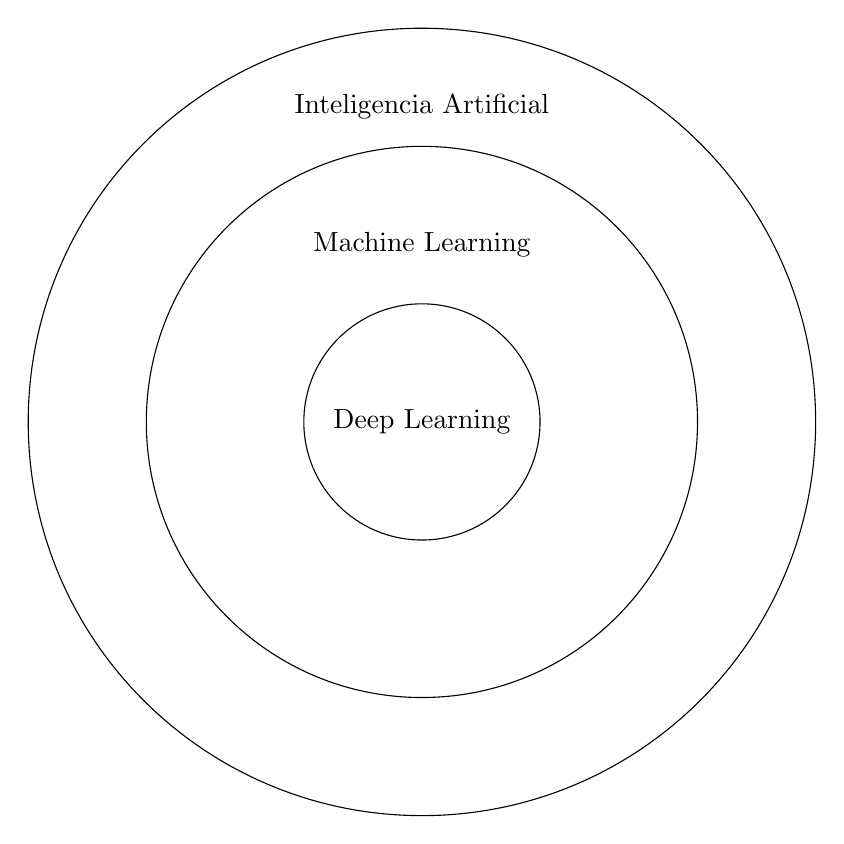
\begin{tikzpicture}
        % Outer circle
        \draw (0,0) circle (5cm);
        
        % Inner circles
        \draw (0,0) circle (3.5cm);
        \draw (0,0) circle (1.5cm);
        % \draw (0,0) circle (0.5cm);
        
        % Labels
        \node at (0,4) {Inteligencia Artificial};
        \node at (0,2.25) {Machine Learning};
        \node at (0,0) {Deep Learning};
    \end{tikzpicture} 
\end{center}

\begin{tcolorbox}[colback=gray!5!yellow!40,colframe=gray!75!black]
    \noindent\textbf{Primeras ''Inteligencias Artificiales'' a crear van a estar enfocadas en Machine Learning.}
\end{tcolorbox}

\noindent
\textbf{Elementos para el aprendizaje de la IA:} La IA requiere de fuentes de datos para entrenarse a si misma. Algunas fuentes de datos son:

\begin{itemize}
    \item kaggle
    \item sklearn
    \item visualdata.io
\end{itemize}


\subsection{Python}
Python es un lenguaje de programación de alto nivel, interpretado y orientado a objetos. Es un lenguaje muy versátil y fácil de aprender, por lo que es muy utilizado en el desarrollo de aplicaciones web, en la ciencia de datos, en la inteligencia artificial, entre otros. Python es un lenguaje de programación muy popular en la actualidad, por lo que es muy probable que ya hayas escuchado hablar de él.

\subsubsection*{Librerías de Python}
Python cuenta con una gran cantidad de librerías que facilitan el desarrollo de aplicaciones en diferentes áreas. La forma de importar una librería en Python es la siguiente:
\begin{lstlisting}
    import numpy as np
    import pandas as pd
\end{lstlisting}

\subsubsection*{Uso de tipos de datos}
Python es un lenguaje de programación que cuenta con varios tipos de datos, como enteros, flotantes, cadenas, booleanos, entre otros. A continuación se muestra un ejemplo de cómo se pueden utilizar estos tipos de datos en Python:
\begin{lstlisting}
    x = 29
    s = "hola"
    f = 15.9
    x = False

    print(x)
    print(s)
    print(f)

    print(s+str(f))
    print(s,f)

    # Variables y Operadores
    a = 10
    b = 5
    suma = a + b
    print(f"La suma es: {suma}")  # Output: La suma es: 15

    # Ciclos y condiciones
    for i in range(5):
        if i % 2 == 0:
            print(f"{i} es par")
        else:
            print(f"{i} es impar")

    a = 45.7875454
    print("El valor es {:.3f}".format(a))
\end{lstlisting}

\subsubsection*{Funciones y uso de parámetros opcionales}
En python se pueden definir funciones de las cuales existen dos tipos de parámetros, los obligatorios y los opcionales. Los parámetros opcionales son aquellos que tienen un valor por defecto y no es necesario pasarlos al llamar la función. A continuación se muestra un ejemplo de cómo se pueden definir funciones en Python:
\begin{lstlisting}
    # Definiendo una función
    def saludo(nombre):
        return f"Hola, {nombre}!"
    
    print(saludo("Jazna"))  # Output: Hola, Jazna!

    # Función con parámetro opcional
    def f(x, y = 4):
        return x + y

    print(f(2))
    print(f(2,8))

    # Función con multiples parámetros opcionales
    def f(x, y = 4, z = 5):
        return x + y + z

    f(3) # Un parámetro de entrada
    f(7, z = 9) # Dos parámetros de entrada con uno opcional (x)
\end{lstlisting}

\subsubsection*{Colecciones de datos}
En python a los arrays se les llama listas, ademas de estos existen los diccionarios y las comprensiones de listas. A continuación se muestra un ejemplo de cómo se pueden utilizar estas colecciones de datos en Python:
\begin{lstlisting}
    # Listas
    lista = [1, 2, 3, 4, 5]
    print(lista[0])  # Output: 1

    # Diccionarios: Colección de datos que se almacenan 
    # en pares clave-valor
    diccionario = {'nombre': 'Ana', 'edad': 25}
    print(diccionario['nombre'])  # Output: Ana

    # Comprensiones de listas: Forma concisa de crear listas al usar []
    cuadrados = [x**2 for x in lista] # Elevar al cuadrado cada elemento 
    print(cuadrados)  # Output: [1, 4, 9, 16, 25]
\end{lstlisting}

\subsubsection*{Bibliotecas para ciencias de datos}

\begin{lstlisting}
    ## Numpy

    lista = [15,20,60,89,45,78,30]
    print("El promedio es {:.2f}".format(np.mean(lista)))
    print("La desviacion estandar es {:.2f}".format(np.std(lista)))
    print("La mediana es {:.2f}".format(np.median(lista)))
    print(f"El valor maximo es {np.max(lista)} y esta en el indice 
    {np.argmax(lista)}")
    print(f"El valor minimo es {np.min(lista)} y esta en el indice 
    {np.argmin(lista)}")

    # Crear un array
    arreglo = np.array([1, 2, 3, 4, 5])
    print(arreglo * 2)  # Output: [ 2  4  6  8 10]

    # Operaciones matematicas
    matriz = np.array([[1, 2], [3, 4]])
    print(np.dot(matriz, matriz)) # Output: [[7 10] [15 22]]


    ## Pandas

    # Crear un DataFrame
    datos = {'Nombre': ['Ana', 'Luis', 'Marta'], 'Edad': [25, 32, 22]}
    df = pd.DataFrame(datos)
    print(df) # Output: Nombre Edad 0 Ana 25 1 Luis 32 2 ... (tabla)

    # Filtrar datos
    mayores_25 = df[df['Edad'] > 25]
    print(mayores_25) # Output: Nombre Edad 1 Luis 32 (tabla)


    ## Matplotlib
    import matplotlib.pyplot as plt

    # Grafico simple
    x = [1, 2, 3, 4, 5]
    y = [2, 4, 6, 8, 10]
    plt.plot(x, y)
    plt.title('Grafico de ejemplo', fontsize=16, fontweight="bold")
    plt.xlabel('x', fontsize=14, fontweight="bold")
    plt.ylabel('y', fontsize=14, fontweight="bold")
    plt.show() # Output: Grafico de ejemplo 
\end{lstlisting}

\newpage
\subsubsection*{Manipulación de datos}

\noindent → Preprocesamiento: Hace referencia a la limpieza y transformación de los datos para que puedan ser utilizados por los algoritmos de aprendizaje automático.
\begin{lstlisting}
    from sklearn.preprocessing import StandardScaler

    # Datos de ejemplo

    datos = [[1, 2], [3, 4], [5, 6]]
    scaler = StandardScaler()
    datos_normalizados = scaler.fit_transform(datos)
    print(datos_normalizados)
\end{lstlisting}

\begin{center}
    \textbf{Estandarización}
    \begin{equation*}
        \textnormal{Valor estandarizado} = \frac{\textnormal{Original} - \bar{x}}{\textnormal{STD}} 
    \end{equation*}
\end{center}
 
\noindent → Ingeniería de características: Consiste en la creación de nuevas características a partir de las características existentes para mejorar el rendimiento de los algoritmos de aprendizaje automático (machine learning).
\begin{lstlisting}
    from sklearn.preprocessing import PolynomialFeatures

    # Crear caracteristicas polinomicas
    poly = PolynomialFeatures(degree=2) # Grado 2 para el polinomio
    datos = [[2, 3]]
    print(poly.fit_transform(datos))  # Output: [[1. 2. 3. 4. 6. 9.]]
\end{lstlisting}
\begin{align*}
    \textnormal{Características polinómicas} = [\textnormal{bias}, x_1, x_2, {x_1}^2, x_1 \cdot x_2, {x_2}^2]
\end{align*}

\subsubsection*{Algebra lineal}

\noindent → Producto cruz entre vectores
\begin{lstlisting}
    # Definir dos vectores
    x_vector = np.array([1, 2, 3])
    y_vector = np.array([4, 5, 6])
    
    # Calcular el producto punto
    producto_punto = np.dot(x_vector, y_vector)
    
    print("Producto Punto:", producto_punto)
\end{lstlisting}

\noindent → Multiplicación entre matrices: Las redes neuronales utilizan la multiplicación de matrices para realizar operaciones matemáticas.
\begin{lstlisting}
    # Definir dos matrices
    matriz_a = np.array([[1, 2, 3],
                         [4, 5, 6]])
    matriz_b = np.array([[7, 8],
                         [9, 10],
                         [11, 12]])
    
    # Calcular la multiplicacion de matrices
    resultado = np.dot(matriz_a, matriz_b)
    
    print("Multiplicacion de Matrices:\n", resultado)
\end{lstlisting}

\noindent → Descomposición en valores singulares: Reducción de la dimensionalidad para utilizarse en métodos como PCA y tratamientos de datos de la IA. Su uso es mas común en Deep Learning.
\begin{lstlisting}
    # Crear una matriz
    matriz = np.array([[1, 2, 3],
                       [4, 5, 6],
                       [7, 8, 9]])

    # Aplicar SVD
    U, S, Vt = np.linalg.svd(matriz)

    print("Matriz U:\n", U)
    print("Valores singulares S:\n", S)
    print("Matriz V traspuesta:\n", Vt)
\end{lstlisting}

\noindent → Tensores y escalares: 
\begin{lstlisting}
    # Escalar (Tensor de rango 0)
    escalar = 29

    # Vector (Tensor de rango 1)
    vector = np.array([1, 2, 3])
    print("Vector\n", vector)

    # Matriz (Tensor de rango 2)
    matriz = np.array([[1, 2, 3], [4, 5, 6], [7, 8, 9]])
    print("Matriz\n", matriz)

    # Tensor de rango 3
    tensor_3d = np.array([[[1, 2], [3, 4]], [[5, 6], [7, 8]], 
                          [[9, 10], [11, 12]]])
    print("Tensor 3D\n", tensor_3d)
\end{lstlisting}

\noindent → Operaciones entre vectores: 

\noindent → Funciones unviersales:

\noindent → Manipulacion de forma:




\newpage
\section{Matemáticas aplicadas a la IA}

\newpage
\section{Deep Learning}

\newpage
\section{Machine Learning}

\end{document}
